\section{Lo Zooster}

E' un' infezione da riattivazione.

Il virus è lo stesso della varicella, infatti si chiama \textbf{VIRUS
VARICELLA ZOOSTER.}

E' un' infezione secondaria di una varicella acquisita in genere in età
infantile.

Colpisce prevalentemente gli adulti, vi è anzi un incremento progressivo
a partire dai 50 anni per decennio come possibilità di espressione di
questa infezione latente.

La relazione tra varicella e zoster è stata ampiamente documentata.

Le esperienze di vaccinazione hanno utilizzato il liquido di vescicola
di pazienti con zoster su bambini a cui è comparsa la varicella, l'
identificazione di DNA virus nei gangli spinali di soggetti con anamnesi
di varicella e la possibilità di verificare con le tecniche moderne il
virus in corso di riattivazione.

I requisiti affinchè si slatentizzi il virus presente nell'organismo
sono legati:

\begin{itemize}
\item[1.]
  ad una pregressa infezione da varicella nell' età infantile
\item[2.]
  alla bassa risposta cellulo-mediata.
\end{itemize}
  L' espressione è a livello cutaneo con vescicole localizzate lungo un
  dermatomero, sempre dolorose spesso, accompagnate da febbre. La febbre
  non è costante, il dolore sì.

  Nella riattivazione da Zooster sono importanti:

\begin{itemize}
\item
  l' età (dopo i 50 anni)
\item
  l' immunodepressione
\item
  l' esposizione intrauterina (fattore di rischio e saranno gruppi a
  rischio)
\item
  l' aver acquisito la varicella al di sotto dei 2 anni
\end{itemize}
  Il percorso del VZV ha come destinatarie le fibre sensitive, cioè le
  radici posteriori, quindi una volta acquisita l' infezione da
  varicella resta latente anziché liberarsi, resta nei gangli spinali e
  nei nervi cranici e poi si esprime a livello del dermatomero che è
  innervato da uno specifico nervo sensitivo, dove compare un
  arrossamento (area eritematosa) con vescicole, che possono essere
  precedute da dolore ancor prima dell' espressione cutanea oppure il
  dolore può essere tardivo, successivo a queste. Il dolore è molto
  forte, tanto da dare il nome popolare di ``Fuoco di Sant' Antonio''.

\subsection{Aspetti clinici}

  Alcuni importanti in termini di gravità.

  Decorso variabile in base ai deficit immunitari: i soggetti con
  problemi di risposta immunitaria specialmente cellulo-mediata sono a
  rischio di \textbf{disseminazione e viremia} (10-40\%) dello Zoster,
  il quale si riattiva.

  Una sede importante e pericolosa è data dallo \textbf{Zoster
  oftalmico} con il coinvolgimento del trigemino, presente circa nel
  20\% dei casi di Zoster.

  Possono esserci ulteriori complicazioni in circa il 50\% dei soggetti
  con Zoster oftalmico, in cui si presente una \textbf{cheratite
  neurotrofica.}

  Può coinvolgere il SNC con \textbf{deficit motori di origine
  trasversa, paralisi del facciale, neuriti acute.}

  Altro aspetto importante è rappresentato dalla \textbf{nevralgia
  post-erpetica}, sindrome neuropatica dolorosa che si sviluppa in un
  18- 30\% dei casi dopo la guarigione dal rash cutaneo: dolore
  estremamente forte di difficile controllo.

  Tarda almeno un mese a comparire rispetto ai sintomi dello Zoster e
  aumenta come incidenza dopo i 60 anni e più aumenta l' età, più forte
  è il dolore. E' difficile da trattare e può persistere per oltre un
  anno. Quindi \textbf{il DOLORE è l' elemento che caratterizza l'
  infezione da Herpes Zoster.}

\subsection{Accertamento diagnostico}

  Virus coltivati e tecniche di biologia molecolare moderne che
  accelerano i tempi, così come è possibile la sierologia dell' avvenuta
  infezione.

  Esistono una serie di farmaci anti Herpes che sono \textbf{inibitori
  della sintesi del DNA} attraverso vari meccanismi, documentati in
  termini d' efficacia nelle varie infezioni erpetiche nell' adulto,
  mentre nel bambino non ci sono molti dati.

\subsection{Epidemiologia}
  E' presente in tutti i territori, forse un po' di più nelle zone
  temperate; non c'è una differenza stagionale, mentre c'è una forte
  differenza in base all'età (la più colpita è intorno ai 50 anni, con
  la probabilità che aumenta all'aumentare di ogni decennio).

  La sede più frequente è il torace (dove si esprime nel 50\% dei casi),
  diversamente può colpire il viso e le aree lombo-sacrali e anche la
  zona dell'occhio.

  Negli Stati Uniti, dati molto recenti segnalano un milione di casi l'
  anno (incidenza estremamente elevata); in Europa si stima che circa
  3-4/1000 persone l' anno esprimono lo Zoster, con un rischio che
  aumenta con l' età e la probabilità che una persona abbia un episodio
  nella vita è del 20\%; se calcoliamo solo la popolazione oltre i 50
  anni,la probabilità diventa di 1:2, cioè il 50\% (quindi è molto
  frequente).

\subsection{Modalità di trasmissione}

  E' molto contagiosa, sebbene un po' meno della varicella. Un problema
  nuovo è il rischio d' infezione uomo-uomo del personale d'assistenza.

  La trasmissione principe è certamente il \textbf{contatto diretto} tra
  lesioni cutanee ricche di virus ad elevata concentrazione e un
  soggetto suscettibile, cioè che non ha mai avuto un' infezione da
  varicella. L'infettività permane finchè il soggetto non ha
  cicatrizzato tutte le lesioni, cioè nel momento della cicatrizzazione,
  che avviene dopo circa una decina di giorni, la lesione non è più
  infettante e finchè non sono cicatrizzate tutte le lesioni il soggetto
  resta infettante.

  \textbf{L' espressione clinica del contagio è varicella}, non Zooster:
  quindi il VZV per contagio diretto o per via aerea provoca varicella.

  \textbf{Via aerea}: stanno documentando sempre più questa possibilità
  di trasmissione, cioè la liberazione nell'aria dal liquido della
  vescicola che è fortemente ricco di virus e che permette il contagio
  di persone suscettibili.

\subsection{Prevenzione}
  Possibilità di prevenzione:
  \begin{itemize}
  
\item
  prevenzione generale ed educazione sanitaria
\item
  prevenzione mirata con il VACCINO: da pochi anni esiste un vaccino
  specifico contro il virus varicella zoster che si chiama \textbf{HZ}
  (sigla), somministrato in un' unica dose sopra i 50 anni (nei bambini
  invece utilizziamo il virus per la varicella) s.c. (sottocutanea). È
  un vaccino vivo e attenuato (ceppo oka).
  \end{itemize}

  Il VACCINO presenta come \textbf{CONTROINDICAZIONI:}
\begin{itemize}
\item \textbf{ipersensibilità} ai principi attivi
\item essendo un virus vivo attenuato, trova tutte le esclusioni di questo
  tipo di vaccini: per esempio la \textbf{gravidanza} (anche se
  considerando l'età in cui una donna è fertile il rischio di sviluppare
  lo zoster è più basso - rischio dopo i 50 anni- ma comunque non è
  trascurabile)
\item qualunque \textbf{deficit immunitario}, in particolare cellulo -
  mediato , così come le infezioni sintomatiche da \textbf{HIV} e la
  presenza di \textbf{malattie gravi.}
\end{itemize}
  Le \textbf{REAZIONI AVVERSE} sono reazioni globali dovute alla
  somministrazione e si possono anche esprimere con una moderata
  malattia (una varicella lieve).

  L' efficacia è dimostrata dai dati che disponiamo: i tempi sono
  abbastanza brevi dal momento della vaccinazione e c'è una
  \textbf{riduzione dello Zoster nel 50\% dei casi, una riduzione della
  nevralgia post- erpetica nel 67\% dei casi e una riduzione forte della
  gravità della malattia.}

  Per quanto riguarda la durata dell'immunità abbiamo pochi dati, solo
  di qualche anno: dopo un anno vi è una caduta del titolo anticorpale,
  che però si assesta e rimane stabile per 3 anni (si vedrà poi nel
  tempo quanto dura la protezione).

  Il vaccino contro lo Zoster non si può dare ai bambini (la scheda
  tecnica prevede la vaccinazione solo dell'adulto), a differenza del
  vaccino per la varicella. Uno dei motivi è che è molto più forte (non
  confondere i due percorsi): nell'infanzia c'è il vaccino della
  varicella, nell' anziano e nell'adulto suscettibile il vaccino per l'
  Herpes.

\section{Citomegalovirus}

\subsection{Eziologia}
  E' un herpes virus a DNA, rivestito da pericapside, fragile,
  parzialmente eliminabile dall' ambiente dai disinfettanti,
  specie-specifico.

  Conosciamo solo un antigene con varianti intratipiche. Dà luogo ad un'
  immunità sia umorale che cellulo-mediata, virus coltivabile seppure
  con un ciclo replicativo lento; anch'esso da vita ad un' infezione
  latente e quindi prevede la possibilità di una riattivazione.

  L' infezione può essere dovuta sia ad un Citomegalovirus esogeno che
  infetta un soggetto suscettibile, quindi diventa sieropositivo e
  abbiamo l' infezione primaria ma possiamo anche avere una reinfezione
  del sieropositivo a distanza di tempo oppure una riattivazione di
  virus latente.

  La \textbf{CAPACITA' DI LATENZA} successiva all'infezione primaria è
  legata al fatto che il virus è in grado di permanere nell'ospite nelle
  cellule mononucleate del sangue, nei tubuli renali, nelle ghiandole
  salivari e qui rimane silente o latente nel senso di ferma o di
  lentamente replicativa, ma può essere slatentizzata in varie
  circostanze. Il virus latente è comunque infettante.

  L' impatto sull'immunità: i meccanismi della latenza non sono noti,
  però si sa che il virus è in grado di deprimere l' espressione degli
  antigeni del complesso maggiore di istocompatibilità e questo
  probabilmente contribuisce alla persistenza del virus nell'organismo.

  La riattivazione è legata principalmente a condizioni di
  immunodepressione, ma anche in corso di altre malattie come quelle
  virali oppure in caso di trattamento con chemioterapici che rendono
  più fragile l'ospite e facilitano la slatentizzazione.

\subsection{Aspetti clinici}

  Le conseguenze dell'infezione citomegalica sono diverse a seconda che
  colpiscano l' adulto, il nuovo nato (perinatale) oppure il prodotto
  del concepimento.

  Nell'adulto, se immunocompetente, l' infezione è normalmente
  asintomatica o lieve; il problema insorge quando ci sono deficit
  immunitari, dove si esprime in forma grave (specialmente in caso di
  deficit cellulo-mediati).

  Nei giorni attorno all'evento nascita può dar luogo ad una malattia
  neonatale, ma spesso è asintomatico.

  Se viene colpita la madre con una prima infezione in gravidanza si
  hanno vari casi:
\begin{itemize}

\item
  può esserci un \textbf{danno fetale},
\item
  può essere un bambino sano, ma che presenterà \textbf{manifestazioni
  nel corso degli anni},
\item
  in molti casi è \textbf{asintomatico}.
\end{itemize}
  L' \textbf{AZIONE PATOGENA} del virus deriva da alcune caratteristiche
  specifiche:
  \begin{itemize}
  
\item
  è in grado di \textbf{evadere la neutralizzazione} perché passa da
  cellula a cellula senza uscire e quindi senza poter essere aggredito
  dalle difese dell'ospite. Ha una breve fase viremica.
\item
  Spesso è \textbf{rivestito e protetto da microglobuline}.
\item
  In più abbiamo delle \textbf{piccole, ma importanti differenze
  antigeniche tra i ceppi} che offrono un escamotage per impiantarsi.
  \textbf{Induce i recettori per il frammento Fc delle Ig}, quindi
  bloccando in parte l' azione di difesa. \textbf{Provoca l'
  immunosoppressione, deprimendo e sopprimendo i linfociti T e
  bloccandone l' attività. }
\item
  E' in grado di innescare fenomeni di \textbf{autoimmunità }
\item
  infine \textbf{favorisce le sovra infezioni batteriche} perché in
  grado di esporre dei recettori generici, che legano una molteplicità
  di batteri e quindi le sovra infezioni sono facili e frequenti.
\end{itemize}
  Entra per \textbf{via aerea}, si diffonde attraverso il sangue con una
  \textbf{breve fase viremica} e questo gli consente di arrivare nelle
  varie sedi prioritarie (oltre alle ghiandole salivari anche nelle
  cellule renali dove si realizza una lunga replicazione).

  La \textbf{CLINICA} è in funzione dell'età e dello stato immunitario,
  del fatto che si tratta di prima infezione e reinfezione e ovviamente
  della carica infettante.

  Nell'adulto quando non è asintomatica, è lieve e c'è una \textbf{forma
  simil-mononucleosica} ed eccezionalmente ci possono essere anche
  \textbf{danni a carico della retina o poliviscerali.}

  \textbf{Importante invece se colpisce un ospite con deficit
  immunitari, specie cellulo-mediati, dove la più frequente in assoluto
  è la POLMONITE da Citomegalovirus} che è estremamente grave,poi c'è
  \textbf{epatite, retinite ed encefalite}.

  Per quanto riguarda la sindrome mononucleosica si ritiene che circa un
  quarto dei casi di sindromi siano legate all'infezione citomegalica.
  Ovviamente l' espressione è diversa dal punto di vista clinico dalla
  forma classica (da Epstein-Barr) perché l' angina è scarsa ed è minore
  l' interessamento linfonodale.

  L' apparato respiratorio è più fragile e coinvolto nel paziente
  immunodepresso, specie se ha subito un \textbf{trapianto d' organo} e
  può andare incontro ad una \textbf{polmonite estremamente grave e
  anche letale} e può anche comportare il \textbf{rigetto.}

  Nell'\textbf{HIV positivo} è frequente soprattutto la
  \textbf{retinite}.

  Molti studi sembrerebbero indicare un \textbf{tropismo endoteliale}
  per il Citomegalovirus e quindi correlato a \textbf{vasculopatie post
  trapianti e ad arterosclerosi.}

  Un gruppo a rischio è rappresentato dai \textbf{trasfusi} che possono
  presentare una \textbf{sindrome mononucleosica virale e la polmonite.}

  Si calcola un \textbf{2-3\% di rischio per unità di sangue trasfuso}
  (c'è un attento controllo delle unità di sangue, quindi è un rischio
  molto generico).

  Un altro gruppo a rischio è rappresentato dai \textbf{prematuri che
  richiedono trasfusione} per la loro prematurità; abbiamo un
  \textbf{tasso di mortalità del 20\%.}

  Il peso dell'\textbf{infezione congenita} è relativamente basso: l'
  infezione si realizza nello \textbf{0,5-2\% di tutti i nati (dato
  mondiale).} All'interno di questo 0,5-2\% \textbf{la probabilità che
  sia sintomatica è del 10\% e un 10\% di questi sintomatici rischiano
  la morte.} La prevalenza vede quindi un 90\% senza alcun segno, però
  possiamo avere \textbf{sequele tardive} in una parte di questi
  asintomatici alla nascita, che presenteranno problematiche in corso di
  sviluppo. Anche l' \textbf{infezione perinatale} è prevalentemente
  asintomatica, solo un \textbf{5\% dei casi presenta una
  sintomatologia.}

  Nell' infezione congenita il danno, quando non è asintomatico, si
  esprime con \textbf{microencefalia, retinite, encefalite e sequele
  neurologiche, sordità (sempre più documentata) e manifestazioni
  tardive a carico dell' occhio, dell' udito, ritardo mentale (QI
  ridotto) e disturbi comportamentali.}

  Interessante è la differenza tra casi reali documentati a livello
  internazionale (dati americani) di principali cause di danno nel
  neonato e la percezione del rischio nella popolazione nei confronti
  delle stesse: in effetti si vede la frequenza di danno tra i primi da
  citomegalovirus, mentre il danno da HIV è contenuto. La percezione del
  rischio non vede il Citomegalovirus, mentre sente molto il rischio
  dell'HIV. C'è un' inversione di conoscenza e quindi anche di tentativi
  di controllo.

  Sempre più si documenta il peso della sordità a seguito dell'
  infezione congenita da Citomegalovirus (è il \textbf{20\% di tutte le
  cause di sordità).}

\subsection{Trasmissione}
  Presenza nelle \textbf{vie aeree, urina, saliva, sangue ed
  eventualmente organi qualora ci fosse un accertamento post-mortem}.
  Tra le infezioni virali è certamente la più diffusa sul pianeta,
  dimostrata da studi siero epidemiologici, cioè la presenza di Ab in
  varie fasce di età o popolazioni documentano come \textbf{nei paesi
  industrializzati oltre il 50\% degli adulti presentano anticorpi anti
  Citomegalovirus,} il che significa che c'è stata infezione. In alcuni
  paesi arriva anche al 100\%.

  Fattori che favoriscono questa circolazione sono legati a:
  \begin{itemize}
  
\item
  latenza,
\item
  al numero elevato di portatori sani
\item
  alla lunga eliminazione che è presente in molti di questi soggetti d'
  infezione.
\end{itemize}
  In uno studio che ha coinvolto molti paesi sulle condizioni di siero
  positività, per quanto riguarda l' \textbf{Italia} due città nord sud,
  si vede che \textbf{la sieropositività si attesta intorno al 92\%,}
  quindi è un' infezione estremamente diffusa. Nei paesi in via di
  sviluppo arriva anche al 100\%.

  La probabilità di incontrare il virus cresce progressivamente con l'
  età. Le riserve di infezione sono rappresentate dall'uomo perché è
  specie specifico, come malato, ma è importante anche il portatore sano
  (colui che si infetta senza esprimere come nel caso dell'adulto
  immunocompetente). Molto importante come sorgente d' infezione è il
  neonato infetto.

  Le modalità di trasmissione sono legate ai liquidi biologici in cui il
  virus è presente: urina (documentata nel 5\% delle donne gravide),
  saliva, sperma, secrezioni cervicali, latte (via importante nella
  trasmissione perinatale),organi trapiantati, leucociti e sangue.

  L' escrezione è particolarmente lunga sia negli immunodepressi che nei
  bambini che nascano infetti, perché si è riscontrata la positività
  anche a 5 anni dalla nascita.

  Fortissimi fattore è la socializzazione per quanto riguarda l' età
  infantile e gli adulti che li gestiscono.

  \textbf{La trasmissione può avvenire sia per via diretta per contatto
  mucoso (bacio), sia per via sessuale, sia per via verticale}. Ci sono
  anche la \textbf{trasmissione semidiretta e indiretta}. In realtà il
  virus è fragile, però ci sono degli escamotage per far sì che ciò
  possa avvenire in quanto la permanenza nella via aerea è breve (via
  indiretta). Poi abbiamo la \textbf{via parenterale}, prevalentemente
  leucociti, \textbf{attraverso un trapianto d' organo e attraverso le
  urine (via indiretta),} a causa delle quali la contaminazione
  dell'ambiente favorisce la persistenza del virus. Da qui deriva che i
  neonati sono a rischio di infezione citomegalica , sia per modalità
  verticale (placentare o perinatale),sia tramite il latte e sia per
  rapporti interpersonali.

  I bambini per contatto delle secrezioni con altri bambini e/o
  genitori,adulti e parenti e naturalmente gli adulti prevalentemente
  per rapporti sessuali e in seconda istanza per trasfusioni (contagio
  inter umano).

\subsection{Profilassi}
  purtroppo non abbiamo una profilassi mirata, quindi dobbiamo avvalerci
  delle \textbf{manovre di prevenzione} \textbf{di tipo generale}, cioè
  contenimento del contagio e comportamentale (molto importante è l'
  educazione sanitaria, quindi sapere quali sono i modi di trasmissione
  e le sorgenti d' infezione).

  Quindi per l' adulto educazione sanitaria.

  Nello specifico \textbf{nella DONNA GRAVIDA bisogna conoscere lo stato
  immunitario}, perché se, com'è probabile, gli anticorpi sono presenti,
  la donna è tranquilla (perché non è mai stata dimostrata una seconda
  infezione con danni al prodotto del concepimento) (la verifica è un
  elemento chiave come nella Rosolia), fare educazione sanitaria e nel
  caso in cui continui a lavorare, allontanare le attività a rischio.

  Per trapianti e trasfusioni: controllo degli interessati previsto per
  legge, controllo del donatore e prevenzione farmacologica.

  Abbiamo però le \textbf{immunoglobuline}, quindi \textbf{profilassi
  immunitaria passiva che vede la sua logica applicazione nei candidati
  a trapianto d' organo.}

\subsection{Vaccino}
  Molti sono stati i vaccini preparati, studiati e provati, ma
  \textbf{non c'è ancora un vaccino in uso},quindi siamo ancora in
  attesa (perché essendo un herpes virus deve essere non solo efficace,
  ma anche sicuro).

\subsection{Correlazioni importanti}

  Nel trapiantato è possibile la comparsa sia nell'organo che nel
  soggetto ricevente di gravi complicazioni, mediamente nei primi
  100-120 giorni dal trapianto.

  Correlazione Citomegalovirus e AIDS per organi interessati con lesioni
  importanti quali l' ottico,tratto gastroenterico, SNC e polmone. Qui a
  differenza della condizione normale la viremia è prolungata, (nell'
  ospite normale invece è breve)

  Per questo ed altri virus (HIV, enterovirus, polio) c'è una
  facilitazione alla slatentizzazione reciproca.

  La correlazione con l' arteroscelerosi è documentata su popolazioni
  animali.

  Correlazione con il diabete insulino dipendente.

\section{Toxoplasmosi}
  La Toxoplasmosi è un' \textbf{antropozoonosi}, una malattia
  parassitaria tipica del mondo animale che non ha mai colpito l' uomo
  se non a partire dagli anni '40 quando è stata correlata ad un neonato
  che presentava malformazioni. Alcuni anni dopo, proprio in Italia, non
  solo ci sono stati altri casi, ma si è presentata anche la
  toxoplasmosi acquisita dell'adulto: quindi non solo infezione e
  possibilità di danno fetale, ma anche nell'adulto.

  Dal punto di vista eziologico dobbiamo considerare tre forme del
  parassita:

\begin{itemize}
\item
  \textbf{Tachizoita} quando in forma vegetativa intracellulare (sangue
  o cellule);
\item
  \textbf{Trofozoita} (forma vegetativa libera);
\item
  \textbf{cisti tissutale} (o pseudocisti), prima forma di resistenza
  tissutale
\item
  \textbf{oocisti},forma di resistenza ambientale
\end{itemize}
  Si tratta di un parassita endocellulare obbligato che mantiene la sua
  vita attraverso due cicli vitali: uno sessuato che si realizza solo
  nei felidi (il prototipo è il gatto, serbatoio importantissimo) e un
  ciclo asessuato che si svolge negli ospiti intermedi (moltissimi nel
  mondo animale).

  Due sono le forme che colpiscono l' uomo: l' acquisita e la connatale.

  Immagine microscopica con la forma tipica a spicchio di mandarino, la
  cisti tissutale, l' oocisti, il trofozoita e il tachizoita.

  Le due forme di resistenza modica e prolungata nel tempo sono la cisti
  tissutale, che contiene fino a mille bradizoiti, cioè piccoli protozoi
  a lenta replicazione (bradi) più o meno fermi in termini di
  replicazione e l' oocisti dove sono presenti due sporocisti e quattro
  sporozoiti.

  La probabilità d' incontro di questi dipende anche dalla loro capacità
  di resistere nell' ambiente: sia trofozoita che tachizoita sono
  fragili, resistono poco nell' ambiente e anche ai succhi gastrici. La
  cisti tissutale invece è quella di latenza nel periodo d' infezione
  dell' uomo ed ha una resistenza maggiore rispetto alle precedenti sia
  all' ambiente che ai succhi gastrici). Poi abbiamo l' oocisti che
  viene eliminata solo dal gatto nell'ambiente dove può rimanere per

  tempi estremamente lunghi: è molto resistente anche agli agenti
  disinfettanti.

\subsection{Ciclo Biologico}

  Nel ciclo biologico fondamentale del Toxoplasma gondii il gatto la fa
  da padrone perché si può infettare da animali intermedi oppure da
  altre oocisti emesse da altri gatti (per esempio sappiamo che il gatto
  si purifica mangiando l' erba e qui possono trovare le oocisti ed
  infettarsi). Nel gatto avviene il ciclo sessuato e una volta terminata
  la replicazione, lo zigote cade nel tratto intestinale,si forma l'
  oocisti immatura che viene eliminata con le feci per oltre due
  settimane. Per diventare infettante la cisti deve maturare e questo
  dipende dalle condizioni ambientali in tempi diversi: è molto veloce
  se la temperatura è medio alta (pochi giorni) oppure rallenta e può
  diventare di quasi un mese a temperature basse intorno ai 10 gradi.

  Tra gli ospiti intermedi interviene anche la specie umana; quindi il
  Toxoplasma ha una vasta varietà di possibilità per sopravvivere
  nell'ambiente: attraverso infezioni di uccelli, ratti ed animali vari
  e anche trasportato passivamente da vettori. Può infettare animali
  vertebrati come ovini, suini (importante), equini, caprini e può
  arrivare all'uomo con varie modalità, sia con i vegetali per
  contaminazione dell'ambiente, sia animali e la donna, se infettata nel
  periodo gravidico, può infettare il prodotto del concepimento con
  danni particolarmente seri.

  L' uomo si può infettare dall'ambiente per attività di giardinaggio,
  agricoltura ecc..

  Il parassita è presente in tutto il pianeta e la sua sopravvivenza è
  garantita da più di una serie di fattori: non uccide l' ospite,
  infetta moltissime specie (mammiferi, uccelli, rettili, molluschi),
  resta silente nell'ospite anche per anni finchè un predatore non
  acquisisce l' infezione (sopravvivenza negli animali intermedi finchè
  a loro volta non vengono predati).

  L' ospite naturale o definitivo che per noi è il gatto produce un
  numero molto elevato di oocisti per un tempo discretamente lungo.

  Può essere trasmesso per via trans-placentare, quindi un ulteriore
  vantaggio, e per ultimo non necessita di un ciclo sessuato per
  vivere,ma gli basta quello asessuato (ha tutte le forme di sicurezza
  per mantenere la specie).

\subsection{Aspetti clinici}

  Nell'uomo la \textbf{forma acquisita di toxoplasmosi nell'adulto è per
  lo più asintomatica nell'80\% dei casi ed è documentata dalla comparsa
  di anticorpi specifici.}

  Quando si presenta clinicamente, segue tre stadi:

\begin{itemize}

\item[1.]
  \textbf{FASE ACUTA}: dura una decina di giorni con replicazione e
  diffusione ad ondate successive via linfo-ematica, quindi parassitemia
  e potenziale arrivo alla placenta e al feto;
\item[2.]
  \textbf{FASE INTERMEDIA}: legata alla risposta dell'ospite con la
  produzione di anticorpi e quindi il parassita si ritira in organi
  privi o con poche cellule immunocompetenti;
\item[3.]
  \textbf{FASE DI CRONICIZZAZIONE TISSUTALE}: si esprime negli organi
  suddetti con la formazione delle pseudo cisti o cisti tissutali e qui
  può permanere a lungo, ma può anche slatentizzarsi, rompersi e dare
  vita ad un' ulteriore infezione.
\end{itemize}
  \textbf{L' espressione clinica più frequente nel giovane (che
  rappresenta il 15\% delle forme) è quella linfonodale}, la meno grave,
  ma può dare anche forme più gravi,generalizzate, curabili ma
  sicuramente impegnative \textbf{simil rickettiosica, parenchimatosa,
  oculare (corioretiniti).}

  Per quanto riguarda il PRODOTTO DEL CONCEPIMENTO: se la donna non
  immune viene infettata in gravidanza si può esprimere con
  \textbf{aborto o morte neonatale}, \textbf{neonato con toxoplasmosi
  alla nascita, neonato con malformazioni, neonato apparentemente sano
  alla nascita perché può esprimere altri problemi tardivamente o
  neonato sano (la quota maggiore).}

  La gravità della toxoplasmosi connatale è in rapporto:

\begin{itemize}

\item
  Alla \textbf{virulenza del ceppo }
\item
  All'\textbf{immunità della madre} (quindi se è la prima infezione
  oppure no)
\item
  Al \textbf{periodo dell'infezione} (1\textsuperscript{o}, 2\textsuperscript{o} o 3\textsuperscript{o} trimestre della
  gravidanza)
\end{itemize}
  La frequenza di trasmissione della toxoplasmosi primaria nella
  gestante è inversamente proporzionale al periodo: è più probabile che
  ci sia passaggio parassitario nell'ultimo periodo,però la gravità è
  all'opposto. Quindi nel primo periodo è meno probabile che ci sia
  passaggio, ma se passa è più grave (1\textsuperscript{o} trimestre), seguito dal 2\textsuperscript{o} e
  poco nel 3\textsuperscript{o}. Frequenza e gravità sono inversamente proporzionali:
  minima frequenza nel primo periodo, ma massima gravità; massima
  frequenza nell'ultimo periodo,ma minima gravità (diversamente dalla
  Rosolia).

  Il danno fetale si esprime:

\begin{itemize}
\item
  O con \textbf{tetrade classica}: microcefalia, calcificazioni
  cerebrali, idrocefalia e corioretinite pigmentaria, danni a carico
  dell'occhio e ritardo psicomotorio, anche tardivo;
\item
  nel 2\textsuperscript{o} trimestre può,seppur eccezionalmente,ancora esprimersi come
  tetrade classica oppure manifestazioni neurologiche, espressioni
  quindi che si rendono evidenti dopo la nascita nell'età scolare;
  nell'ultimo trimestre o c'è una toxoplasmosi alla nascita oppure non
  c'è nulla o ci sono lesioni epatiche o altre espressioni di minore
  impatto, ma non gravi malformazioni.
\end{itemize}

\subsection{Epidemiologia}
  E' una parassitosi diffusa in tutto il pianeta, documentata dal
  presenza di anticorpi che risultano in alcune popolazioni rasentare il
  100\%, legata ad aspetti culturali.

  Molto frequente è l' infezione negli immunodepressi ( tant'è che
  all'inizio era considerata una delle cause della malattia) e nel
  trapiantato.

  La frequenza è condizionata da una serie di fattori:
  \begin{itemize}
  
\item
  Dall'\textbf{ambiente climatico}: il clima caldo-umido favorisce il
  protozoo e la sua sopravvivenza e ne accelera la maturazione
\item
  Le \textbf{condizioni igieniche}
\item
  Le \textbf{abitudini alimentari}
\end{itemize}
  Per quanto riguarda la suscettibilità della popolazione femminile
  adulta in Italia, si calcola che un 60\% circa della popolazione in
  età fertile non presenti anticorpi nei confronti del Toxoplasma.

  La diffusione è favorita:

\begin{itemize}
\item
  dalla \textbf{zona} geografica ed in particolare quella
  \textbf{rurale}, che espone più facilmente al contagio (contatto con
  la terra, veterinari )
\item
  dallo \textbf{stretto rapporto con gli animali} (gatti, passeri e
  altri ospiti intermedi) a vita semilibera o libera, che può
  incrementare la possibilità di contagio ma anche la persistenza del
  parassita
\item
  dalle \textbf{abitudini alimentari }
\end{itemize}
  Il Toxoplasma è presente anche negli equini, nei suini (fino ad un
  70\%) che come gli ovini e i bovini rientrano nella nostra
  alimentazione ( carni a rischio).

  Le \textbf{sorgenti d' infezione} sono:

\begin{itemize}
\item
  il \textbf{gatto} (serbatoio)
\item
  l' \textbf{ambiente} (presenza delle oocisti)
\end{itemize}
  \textbf{La modalità di trasmissione:}
  \begin{itemize}
\item
  \textbf{DIRETTA} (quella verticale, transplacentare)
\item
  \textbf{INDIRETTA} (la più importante in assoluto) è l' ingestioni di
  carni crude o poco cotte infettate da pseudocisti (quindi sono
  importanti le abitudini culinarie: popolazioni che mangiano
  tipicamente carni crude come la tartare e il carpaccio o salsicce
  crude, sono molto esposte al contagio), ingestione di oocisti presenti
  nel terreno (durante attività di giardinaggio o attività agricola),
  ingestione di verdure contaminate, fonti di origine animale per
  contatto stretto e rischio sanitario come trapianti d'organo o
  trasfusione infetti (perché c'è una fase parassitemica), incidenti di
  laboratorio ecc\ldots{}
  \end{itemize}

  La frequenza della toxoplasmosi sintomatica connatale a livello
  mondiale è dello 0,1-0,8\%.

  In Italia siamo nel mezzo, quindi allineati con i dati internazionali.
  Sullo 0,4\% può esserci un problema nel 10-30\% dei casi.

\subsection{La diagnosi}
  Oggi ci si basa prevalentemente sulla \textbf{sierologia}, ma c'è la
  possibilità di fare anche un accertamento più approfondito, mediante
  la biologia molecolare e ricerche microscopiche.

  Le indagini sierologiche sono molto utili perché ci danno un quadro
  dell'immunità del soggetto ed andrebbero applicate in modo molto più
  esteso, in particolare sulla popolazione in attività fertile.

\subsection{La prevenzione}
  Per la toxoplasmosi acquisita:
  \begin{itemize}
  
\item
  controllo delle carni e della cottura (carni crude o poco cotte
  rappresentano il 41\% dei casi documentati di toxoplasmosi)
\item
  attenzioni alle mani contaminate dopo aver toccato carni crude:
  importante il lavaggio delle mani e delle suppellettili utilizzate per
  l' allestimento culinario (tra le carni crude: maiale ed agnello)
\item
  anche le carni congelate sono infette perché il congelamento non
  incide sulle pseudo cisti: l' unico momento in cui possiamo sperare
  che si riducano un po' è lo scongelamento. Questo se il congelamento
  non è stato fatto correttamente poiché se non viene fatto alla giusta
  velocità si formano grossi cristalli di ghiaccio nelle cellule che al
  momento dello scongelamento ne causano la rottura massiccia e quindi
  la fuoriuscita del protozoo. In ogni caso la carne congelata è da
  ritenersi infetta.
\item
  lavaggio accurato di frutta e verdura perché si raccoglie sul terreno
  (esempio della fragola, che si trova in basso); i parassiti sono più
  noiosi dei batteri da allontanare, quindi l' acqua deve essere
  disinfettata
\item
  evitare stretti contatti con i gatti
\item
  disinfettare accuratamente gli utensili usati con prodotti chimici
  (ipocloriti, iodio)
\item
  evitare i contatti stretti con tutti gli animali,sia domestici che
  selvatici
  \end{itemize}

  Tutte queste norme valgono anche nella prevenzione della connatale a
  cui aggiungiamo il controllo dello stato immunitario della donna
  gravida, sperando in una conferma dell'immunità (in realtà sarebbe
  molto utile avere questo dato anche prima, nelle donne in età fertile,
  perché sapere di avere anticorpi anti toxoplasma consente di avere la
  tranquillità in assoluto). Nel caso del Toxoplasma peraltro esistono
  dei farmaci utilizzabili nella donna gravida.

  Come \textbf{SCHEMA DI CONTROLLO}:
  \begin{itemize}
  
\item
  se in una DONNA ADULTA non gravida troviamo anticorpi, sappiamo che è
  protetta;
\item
  se è gravida e non abbiamo dati precedenti, attuiamo la ricerca degli
  anticorpi e se risultano negativi si continua a controllare (follow-up
  durante tutto il periodo gravidico) e si attuano tutte le misure di
  profilassi di cui abbiamo parlato in modo ancor più ristretto per
  esempio impedendo il consumo di carni crude (per esempio i salumi,
  perché non abbiamo la certezza della stagionatura, di verdure crude.
  \end{itemize}

  Se invece ci sono degli anticorpi, bisogna vedere quale tipo, perché
  si deve stadiare l' infezione nella donna in gravidanza (capire quando
  è stata infettata):
  \begin{itemize}
  
\item
  se si presentano Ab di classe IgG a basso titolo da sole, è probabile
  che sia di antica memoria (perché sappiamo essere le più resistenti
  nel tempo)
\item
  se invece abbiamo sia le IgG che le IgM allora è probabile che sia una
  borderline, si tratta di vedere a quale periodo gravidico stiamo
  facendo riferimento.
\end{itemize}
  In entrambi i casi è bene attuare un controllo successivo, per vedere
  se sono stabili o se incrementano:

\begin{itemize}
\item
  se ci sono IgG a basso titolo che incrementano siamo nei guai perché
  l' infezione potrebbe essere avvenuta nel periodo gravidico (1\textsuperscript{o}-2\textsuperscript{o}-3\textsuperscript{o}
  mese, perché l' incremento significa che è in fase di replicazione)
\item
  se rimangono stabili ci conferma che è una vecchia infezione,superata,
  che ha immunizzato
\item
  se ci sono Ig ad alto titolo significa che l' infezione è recente: in
  questi casi, com'è documentato dalle riviste di Ostetricia, c'è la
  possibilità di usare alcuni prodotti farmacologici
\end{itemize}

\section{Infezioni che portano a meningite}
  I principali attori tra i batteri responsabili di meningiti sono
  Meningococco, Pneumococco ed Haemophilus Influenzae di tipo B, che
  rappresentano il 70\% dei casi di meningite, specie nell' infanzia. Ce
  ne sono altri e poi i virus.

\subsection{L'infezione meningococcica}
  E' spesso asintomatica e si può presentare in un' ampia varietà di
  forme cliniche, lievi fino alle più gravi: dalla meningite della alte
  vie fino alla cerebrospinale e a forme settiche fulminanti.

  Oggi è meno temibile rispetto al passato per quanto riguarda la
  possibilità d' intervento, poiché abbiamo una terapia efficace, sempre
  che sia tempestiva e adeguata, cioè specifica per il problema.

  Resta peraltro temibile perché il meningococco è molto diffuso, sia
  nei paesi industrializzati che nei paesi in via di sviluppo, perché è
  l' unico tra quelli nominati ad avere un \textbf{andamento epidemico}
  (si esprime in focolai o epidemie nel pianeta) e perché ha la
  t\textbf{endenza ad esprimersi in nuovi siero gruppi}: dalla classica
  forma meningococcica sostenuta dai ceppi prevalenti, quelli che
  definiamo maggiori, che sono \textbf{A,B e C}, si è andato inserendo
  nel contesto epidemiologico l' impatto epidemico dei ceppi minori: lo
  \textbf{Z, l' Y, il W135} (siero gruppi che prima erano poco
  importanti sul piano epidemiologico).

  Ultimo aspetto che la rende un problema di sanità pubblica è il fatto
  che è andata acquisendo nel tempo una \textbf{resistenza sempre più
  forte ai farmaci.}

  Quindi la difficoltà terapeutica e la persistenza dell'infezione.

  Questo fa sì che sul piano di sanità pubblica sia una delle malattie
  nell'occhio del ciclone e per la quale è determinante la prevenzione
  primaria.

\subsubsection{Eziologia}

\begin{figure}[!ht]
\centering
	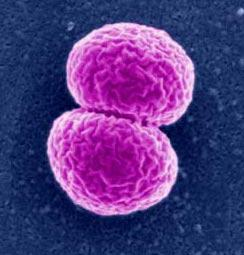
\includegraphics[width=0.3\textwidth]{08/image1.jpg}
	\end{figure}
	
	\begin{figure}[!ht]
\centering
	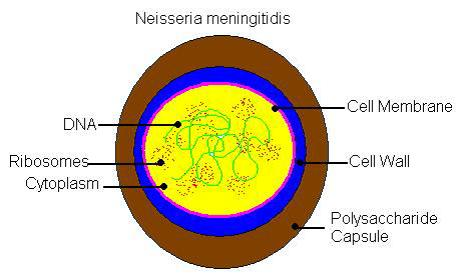
\includegraphics[width=0.4\textwidth]{08/image2.jpg}
	\end{figure}

  Cocco Gram - capsulato (elemento di patogenicità), presenta numerosi
  determinanti antigenici, tra questi i più importanti sono i
  polisaccaridi capsulari, che determinano la nomenclatura, e la
  suddivisione in sierogruppi che sono 13: i primi 3 sono A,B e C e sono
  considerati i maggiori (impatto prevalente sul piano epidemiologico,
  cioè responsabili del 90\% circa dei casi di meningite cerebrospinale
  epidemica), però ci sono anche altri come 29E, H, I, K, L,W135, K,
  Y,Z.

  Esistono poi altre strutture antigeniche, che pero' per noi non hanno
  un importante riflesso in termini di vaccinazione.

  La Neisseria meningitidis è molto labile nell'ambiente esterno,
  facilmente inattivabile dal calore e dalla luce ed anche dagli agenti
  chimici, blandi disinfettanti addirittura. Va inoltre incontro ad
  autolisi.

  E' un \textbf{commensale del rinofaringe, molto comune nella
  popolazione umana}: tutti noi nel corso della nostra vita ci
  infettiamo e ci liberiamo, senza alcun tipo di problema, quindi un
  classico commensale, che in alcune situazioni diventa un patogeno,
  quindi un ampia diffusione.

  Si ritiene che \textbf{dall'1 al 30\% dei soggetti sani sia portatore
  di meningococco}, addirittura in alcune fasce di età la percentuale è
  ancora più elevata.

  Questa condizione di commensalismo è correlata:
  \begin{itemize}
  
\item
  all'età (soprattutto nel bambino)
\item
  alla condizione socio economica
\item
  al ceppo prevalente in quell'area geografica
\item
  non sempre allo stato immunitario della popolazione
\end{itemize}
  Non sempre c'è una correlazione tra stato di portatore ed incidenza di
  malattia;

  La possibilità di espansione è legata alla presenza di un nuovo ceppo
  o ad una carenza anticorpale in quella popolazione nei confronti di
  quel sierotipo.

  Il rischio di sviluppare la malattia è molto più alto nei soggetti a
  contatto con un malato di meningite: quindi è meno rischioso il
  contatto con il portatore rispetto al contatto con il malato
  conclamato.

  Non siamo certi del meccanismo patogenetico (è poco noto), ma sappiamo
  alcune cose che ci aiutano a capire perché sia grave:
  \begin{itemize}
  
\item
  la presenza delle \textbf{proteasi in grado di inattivare le IgA
  secretorie}, delle mucose
\item
  la \textbf{capsula è in grado di aderire alle cellule epiteliali della
  mucosa}
\item
  \textbf{capacità antifagocitaria} sempre grazie alla capsula
\end{itemize}
  La protezione da meningococco è dovuta ad anticorpi battericidi
  specifici; gli Ag capsulari sono fortemente immunogeni e quindi gli Ab
  battericidi mediati dal complemento sono i deterrenti per l' impianto
  del meningococco e quindi di comparsa di epidemie.

  \textbf{Fattori favorenti l' impianto} e quindi lo stato di portatore
  sono:
  \begin{itemize}
 
\item
  stati di sofferenza dell' albero respiratorio (fumo sia attivo che
  passivo)
\end{itemize}
  Il \textbf{passaggio da infezione a malattia} è legato:

\begin{itemize}
\item
  all'ospite:

  \begin{itemize}
  \item
    quando ci sono problemi della cascata del complemento che non
    funziona molto bene
  \item
    in presenza di un' asplenia
  \item
    in presenza di un' immunodepressione grave come in caso di infezione
    da HIV
  \end{itemize}
\item
  a fattori concomitanti:

  \begin{itemize}
  \item
    sono le malattie intercorrenti, specie le virali (è stato
    documentato un aumento d' infezione meningococcica in corso di
    epidemie influenzali, sia di tipo A che di tipo B, ovviamente
    favorente il contagio in condizioni di sovraffollamento con ingresso
    di ceppi nuovi)
\end{itemize}
\end{itemize}
    Il percorso dalla colonizzazione faringea con invasione e
    batteriemia per ingresso nel circolo può comportare lesioni
    endoteliali e superamento della barriera emato-encefalica (si può
    parlare anche di aumento della permeabilità) con edema che causa
    ipertensione endocranica con tutti i danni che può derivare da essa.

    Le malattie da meningococco possono essere sia invasive che non:
    \begin{itemize}
    
\item
  le \textbf{invasive} sono \textbf{meningite, la sepsi indipendente
  oppure meningite più sepsi e poi possono esserci altre sedi come
  polmonite, artrite ed otiti.} Sepsi meningococcica significa invasione
  nel sangue e si può presentare con o senza meningite ed è presente nel
  25\% dei casi.
  \end{itemize}

  I sintomi sono \textbf{rash petecchiale,porpora, ipotensione ed
  insufficienza multi organo.}

  Le cause di sofferenza delle meningi sono tante, quindi la terapia
  specifica deve essere mirata all'agente eziologico, quindi la
  definizione di caso è molto importante.

\subsubsection{Diagnosi di laboratorio}

  E' importante per la terapia mirata ed anche per la prevenzione,
  perché se vogliamo evitare la malattia in soggetti a contatto dobbiamo
  sapere se si tratta di meningococco, pneumococco o altri, perché dire
  meningite è troppo poco.

  Nella diagnosi di laboratorio è importante non solo
  \textbf{l'isolamento}, ma anche \textbf{l'antibiogramma}, cioè la
  conoscenza di sensibilità ai farmaci.

  \textbf{In presenza di terapia antibiotica mirata la letalità della
  meningite è ancora attorno al 7-14\%} ed entra in gioco anche la
  tempestività. La letalità aumenta incredibilmente se c'è sepsi ed in
  più c'è la possibilità di sequele permanenti nei sopravvissuti come
  perdita dell'udito, ritardo mentale ed altri disturbi.

\subsubsection{Epidemiologia}

  Può colpire tutte le età, è \textbf{diffusa in tutto il mondo} e
  abbiamo \textbf{due picchi} caratteristici: \textbf{bambini in età
  prescolare e scolare e giovane adulto} (tant'è che in passato la
  fascia più a rischio in assoluto erano i militari di leva: infatti fu
  loto imposto il vaccino obbligatorio nell'87, a causa dell'ambiente
  sovraffollato e della provenienza della popolazione da tutt'Italia e
  la probabilità di cofattori per l' impianto del batterio e la
  trasformazione in malattia).

\subsubsection{Trasmissione}

  E' a \textbf{trasmissione aerea}, quindi i momenti più critici sono
  fine inverno-inizio primavera.

  La riserva di infezione è l'uomo che è l'ospite naturale. L'uomo è
  anche sorgente in quanto eliminatore, sia come malato, sia come
  portatore sano, che ha un ruolo importante nel mantenimento
  dell'infezione specialmente nella comunità infantile.

  Il numero dei portatori incrementa significativamente nei periodi
  epidemici attorno ad un caso di malattia.

  \textbf{In Italia la condizione di portatore è intorno al 10\%}
  considerando tutte le età.

  La contagiosità dopo la terapia antibiotica dura 24 ore, dopodiche non
  è più contagioso.

  La modalità di trasmissione è per via aerea, per \textbf{contatto
  diretto e semidiretto}, perché resiste poco nell'ambiente.

  La \textbf{zona di maggior diffusione} della meningite è quella
  \textbf{subsahariana}, detta \textbf{cintura africana della
  meningite,} che vede paesi come la Nigeria, l' Etiopia, il Sudan ecc
  come paesi in cui tutti gli anni o in uno o in un altro paese c'è una
  pesante epidemia.

  In questi focolai epidemici si oscilla dai 10 ai 1000 casi per
  100.000, quindi un numero molto rilevante. Inoltre si è calcolato che
  negli ultimi 20 anni ci sono stati oltre 800.000 casi nella stagione
  secca.

  Nelle zone con forti epidemie generalmente prevale il
  \textbf{sierogruppo A}, il più forte, ma è da queste zone che nascono
  i sierotipi minori ed è ciò che è avvenuto negli ultimi anni con il
  W135, che non è mai stato responsabile di fenomeni di meningite nei
  paesi industrializzati, ma che lo è diventato a seguito
  dell'evidenziazione dello stesso in questi territori e poi il
  trasferimento anche nel nostro paese (prima in America). La letalità
  in questi paesi oscilla tra il 10 ed il 50\%.

\subsubsection{Sierogruppi nei vari territori}

  Il \textbf{sierogruppo W135} è nato nelle zone africane (e questo è
  motivo di particolare cautela nei viaggiatori) del culto islamico
  dove,per motivi culturali, si riuniscono milioni di persone all'anno
  provenienti da tutto il mondo: W135 è emerso proprio da uno di questi
  incontri, da cui poi i pellegrini hanno portato il ceppo nei loro
  territori di origine.

  Nei \textbf{paesi industriliazzati si alternano come sierogruppi
  prevalenti il B e il C,} con l' emergenza dei nuovi sierogruppi come
  l' Y, il W135; mentre nei paesi a forti epidemie prevale l' A ed in
  maniera minoritaria gli altri.

  Dati della sorveglianza in Europa segnalano che l' Italia ha un numero
  contenuto di casi, ma ci sono anche nazioni della regione Europa
  (dell'OMS) in cui l'incidenza è estremamente rilevante.

\begin{figure}[!ht]
\centering
	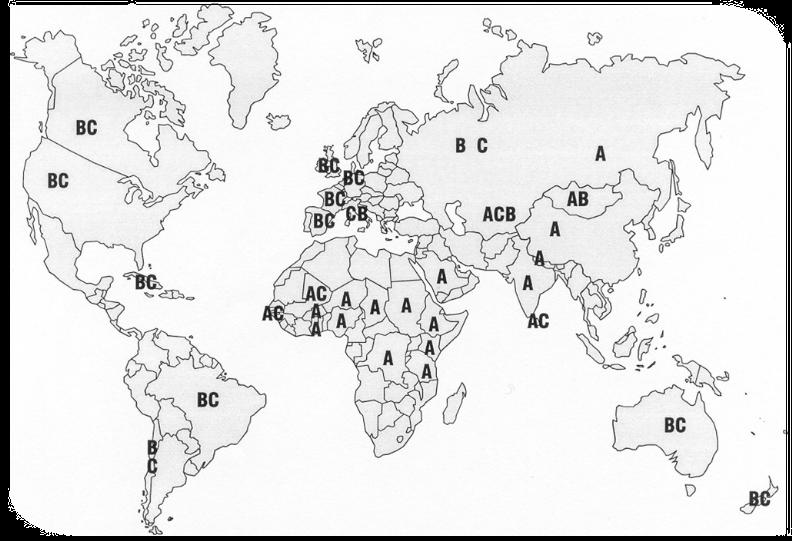
\includegraphics[width=0.8\textwidth]{08/image3.jpg}
	\end{figure}

  La meningite è una \textbf{malattia endemo-epidemica} (in realtà in
  Italia ci sono focolai epidemici; dopo le grandi epidemie del post
  bellico degli anni '60 attualmente, per la possibilità di interventi
  preventivi, si esprime con focolai epidemici regionali, com'è successo
  recentemente in Toscana nel 2005 con il ceppo C).

  \textbf{L' incidenza oscilla in funzione dell'età: }

\begin{itemize}
\item
  è maggiore nei bambini piccoli, dove la malattia è molto più grave;
\item
  si riduce nei bambini in età pre-scolare
\item
  si riduce ulteriormente negli adulti (0,3/100.000 abitanti)
\end{itemize}
  Nel 2005 in Toscana sono stati documentati 38 casi, 9 decessi, ceppo
  prevalente meningoccocco di tipo C. A tutt'oggi nel 2016 sono stati
  segnalati 11 casi.

  In Italia, come in molti paesi industrializzati, i ceppi B e C sono
  presenti costantemente come endemia, quindi ci aspettiamo un numero di
  casi annui.

  Da pochi anni sono comparsi anche l' Y e il W135.

  In Emilia Romagna il peso dell'infezione da meningococco nella torta
  dei responsabili di meningite si è ridotto nel triennio 2007-2009,
  mentre resta pressochè invariato il peso del pneumococco ed aumentano
  gli altri.

\subsubsection{La prevenzione}

\begin{itemize}
\item
  E' soggetta a denuncia obbligatoria di classe II
\item
  E' previsto l' isolamento ospedaliero per la gravità e la possibilità
  di contrarre il contagio
\item
  Sorveglianza sanitaria per contatti e conviventi dai 7 ai 10 giorni
  per verificare l' andamento, quindi non solo per la possibilità di un
  tradursi in malattia, ma anche come controllo di una potenziale
  diffusione e contagio
\item
  La sorveglianza epidemiologica è importante per verificare in caso di
  malattia soggetti suscettibili attorno o sorgenti d' infezione e
  trattamento farmacologico preventivo dei contatti
\item
  Accertamento diagnostico per attuare il vaccino giusto oltre che il
  farmaco
\item
  Disinfezione
\end{itemize}

\paragraph{La profilassi}
  La profilassi mirata si avvale sia del vaccino che dei farmaci (sono
  farmaci per la terapia che possono essere utilizzati a scopo
  preventivo).

  Abbiamo due tipologie come \textbf{preparati vaccinali}:

\begin{itemize}

\item[1.]
  \textbf{I VACCINI POLISACCARIDICI NUDI}:

  \begin{itemize}
  \item
    \textbf{il monovalente A e C} (l' A ci interessa molto poco, perché
    nel nostro territorio non c'è)
  \item
    il \textbf{bivalente A + C}
  \item
    il \textbf{tetravalente A + C + Y + W135}, efficace dopo i 2 anni,
    non funziona bene nel bambino piccolo perché il polisaccaride
    presenta alcuni limiti:

    \begin{itemize}
    \item
      non è timo dipendente quindi non stimolano le cellule T, che sono
      indispensabili per la risposta immunitaria;
    \item
      la risposta immunitaria, almeno nei primi anni di vita è sempre di
      tipo IgM, inizia dopo i 2 anni ed ha una breve durata
    \item
      non stimola le cellule della memoria, quindi non rispondono nè a
      richiami, né a stimoli naturali;

      Quindi non funzionando nel bambino, per proteggerlo è stato ideato
      il vaccino coniugato, cioè in cui il polisaccaride è legato ad una
      proteina carrier, che lo rende fortemente immunogeno e supera il
      problema della timo indipendenza.
    \end{itemize}
  \end{itemize}
\item[2.]
  \textbf{I VACCINI CONIUGATI} (solo da poco disponiamo di un vaccino
  coniugato anche per l'adulto perché il primo vaccino coniugato è stato
  allestito per il neonato perché è una malattia molto grave nel primo
  anno di vita; nell'adulto si usavano esclusivamente i vaccini
  saccaridici).

  Il primo vaccino utilizzato è stato il \textbf{monovalente C}
  ,destinato all'infanzia\textbf{,} efficace sia dopo i 2 anni che
  prima, quindi la somministrazione nel bambino piccolo, se necessaria,
  è di 3 dosi, altrimenti nei tempi successivi all'anno di vita 1 dose.

  In questi ultimi anni in Italia è arrivato il vaccino
  \textbf{coniugato tetravalente,} destinato all' adulto (licenziato in
  Europa nel 2010, è poi arrivato in Italia).

  Indicazioni terapeutiche:utilizzabile dagli 11 anni in su (perché non
  ci sono i dati che lo rendano utilizzabile anche prima).
  Somministrazione: 1 dose.
\end{itemize}
  In questi ultimi anni è stato introdotto il vaccino che mancava contro
  il \textbf{meningococco B} \emph{(informazione non presente sulla
  vecchia dispensa)}\textbf{,} perché il polisaccaride di tipo B
  presenta diversi problemi: innanzitutto perché è molto simile
  all'acido sialico del feto e dell'uomo adulto, quindi questa
  componente microbica non può essere considerata come estranea, quindi
  l' organismo non la riconosce, addirittura può diventare un
  autoantigene, quindi il problema è che al momento della
  somministrazione può dare reazioni immunitarie (tolleranza
  immunogena). Per questo motivo il polisaccaride b non poteva essere
  utilizzato; in più non veniva modificato dalla coniugazione, perciò
  gli studi hanno seguito una strada innovativa molto originale chiamata
  \textbf{REVERSE VACCINOLOGY}, che significa andare a valutare tutte le
  componenti strutturali e non del meningococco, valutando la
  possibilità immunogena delle singole e la capacità protettiva degli
  anticorpi prodotti dalle varie componenti (strada molto interessante,
  ma complessa).

  sono stati studiati diversi tipi di vaccini di varie componenti
  (norvegese, cubana, neozelandese, il prodotto italiano che ha
  identificato 4 componenti).

  Con l' utilizzo di programmi di bioinformatica (si tratta di
  analizzare tutti i geni e le varie componenti) , dopo aver esaminato
  circa 600 geni- proteine per identificare i 4 componenti del vaccino.

  Le 4 componenti che costituiscono il vaccino immunogeno protettivo
  sono:
\begin{itemize}

\item[1.]
  Una proteina di adesione (proteina A) (NadA)
\item[2.]
  Un fattore di legame (fattore H) (fHbp)
\item[3.]
  L' antigene legante l' eparina (NHBA)
\item[4.]
  Una componente presente nella vescicola della membrana esterna (PorA)
\end{itemize}
  Oltre al vaccino è presente anche l' adsorbente;viene somministrato
  per via intramuscolare profonda; c'è l' adiuvante e viene licenziato
  dai 2 anni in su.

\paragraph{Strategia vaccinale in Italia}

  Le motivazioni per l' applicazione del vaccino antimeningococco
  nell'adulto sono:

\begin{itemize}
\item
  gruppi a rischio e per tutti coloro che hanno problemi dei fattori del
  complemento
\item
  soggetti che vivono in zone ad alta endemia
\item
  per contenere episodi epidemici, poiché la velocità di produzione di
  anticorpi è discreta e si può utilizzare il vaccino su soggetti
  suscettibili a contatto con una sorgente d' infezione
\item
  in caso di contatti familiari con casi di meningite
\item
  soggetti splenectomizzati
\item
  reclute militari, perché si trovano in ambienti in cui si concentrano
  soggetti provenienti da aree diverse rendono favorevole la
  contaminazione
\item
  viaggiatori in zone endemiche, specie pellegrini verso zone di culto
  islamico (commistione di ceppi)
\end{itemize}
  E' fortemente consigliato nel bambino piccolo nel primo anno di vita
  per la prevenzione della meningite, non obbligatorio.

  \textbf{Il piano nazionale di prevenzione vaccinale 2018 riprende e
  consolida quello del 2014: tra gli obiettivi prevede di raggiungere e
  mantenere nei nuovi nati e negli adolescenti coperture vaccinali
  superiori al 95\%} per quanto riguarda la protezione da meningococco.

  E' una delle vaccinazioni indicate per chi si reca in zone ad alta
  endemia (Africa: cintura africana e parte mediterranea dell'Africa
  nelle zone del culto islamico).

  Alcuni paesi richiedono la vaccinazione per alcune categorie, in
  particolare per i militari.

  In Italia è obbligatoria per i militari dall'86.

  Secondo le indicazioni dell'OMS è obbligatoria per chi si reca in
  Arabia Saudita, fortemente indicata per chi si reca in tutta una serie
  di paesi, in particolare quelli della cintura africana.

\paragraph{Chemioprofilassi}
  Prevenzione in condizioni di emergenza in caso di forte sospetto o
  certezza di contagio.

  La \textbf{chemioprofilassi} è sempre \textbf{selettiva}: bisogna
  usare al meglio ed al minimo il farmaco a scopi preventivi,perché l'
  incidenza della farmaco resistenza poi crea problemi a tutti, a
  cominciare dalla terapia; quindi è sempre selettiva per i contatti
  stretti: se per esempio si è verificato un caso di meningite a scuola,
  si vaccinano i bambini della classe di quel caso, non tutti i bambini
  della scuola.

  In caso di contatti stretti il rischio di contrarre la malattia è 500
  volte maggiore.

  Il farmaco di scelta è la \textbf{Rifampicina} (mentre in passato
  erano i Sulfamidici che pero' nella quasi totalità dei casi sono
  impossibili da usare per la farmaco resistenza).

  La chemioprofilassi è consigliata a:
  \begin{itemize}
  \item
  contatti familiari
\item
  contatti scolastici molto ristretti
\item
  in bambini molto piccoli (asili nido e scuola materna)
\item
  soggetti che frequentano ambienti molto frequentati e che versano in
  condizioni igieniche scarse (per esempio che frequentano dormitori,
  collegi, caserme..)
\item
  soggetti esposti con il pazienti (medici della rianimazione,
  respirazione bocca a bocca, intubazione endo-tracheale, senza le
  dovute precauzioni\ldots{})
\end{itemize}